\documentclass[12pt]{article}

\usepackage{sbc-template}

\usepackage{graphicx,url}
\usepackage[portuguese]{babel}
%\usepackage[brazil]{babel}   
%\usepackage[latin1]{inputenc} 
 %\usepackage[utf8]{inputenc} 
%\usepackage[brazilian]{babel}
\usepackage[utf8]{inputenc}
\usepackage[T1]{fontenc}
\usepackage{algorithm}
\usepackage{algpseudocode}
\usepackage{indentfirst}
\newcommand{\vars}{\texttt}
\newcommand{\func}{\textrm}
\algnewcommand\And{\textbf{and}}
\algnewcommand\To{\textbf{to }}
\let\oldReturn\Return
\renewcommand{\Return}{\State\oldReturn}


     
\sloppy

\title{Comparando vetores aleatórios em algoritmos de ordenação:. BubbleSort, InsertionSort e Quicksort}

\author{Cleber Soares\inst{1},  Sthefany Oliveira \inst{1}, Victor Souzal\inst{1} }


\address{Faculdade de Computação e engenharia elétrica\\Universidade Federal do Sul e Sudeste do Pará
  (UNIFESSPA)\\
  68505-080 -- Marabá -- PA -- Brasil\\
  \email{\{cleber.soares,sthefany.oliveira,victoor.soouza\}@unifesspa.edu.br}
}

\begin{document} 

\maketitle

\begin{abstract}
  Ordering algorithms are computational methods for organizing and / or ordering a list of numbers or words according to their individualities, they can take care of each case that best suits their needs and then improve certain problems that are related to the retrieval of data in lists, that is, facilitate the search of information. This article presents its implementation, execution and comparative among three sorting algorithms that are: Insertion Sort, Bubble Sort, and Quick Sort. For the purpose of analyzing your results and checking the positives and negatives of each.
\end{abstract}
     
\begin{resumo} 
  Os algoritmos de ordenação são métodos computacionais para organizar e ou ordenar lista de números ou palavras, de acordo com suas individualidades, podem atender cada caso que se adeque melhor a sua necessidade para então melhorar certos problemas que estejam relacionados a recuperação de dados em listas, ou seja, facilitam a busca das informações. Este artigo apresenta a sua implementação, execução e comparativo entre três algoritmos de ordenação que são: Insertion Sort, Bubble Sort, e Quick Sort. Com a finalidade de analisar seus resultados e verificar os pontos positivos e negativos de cada um.
\end{resumo}	


\section{Introdução}
Na computação existem vários tipos de algoritmos que tem diferentes
técnicas para realizar operações de ordenação, tendo como fim facilitar a
busca de conjuntos de dados, seja para organiza-los ou classifica-los em
ordem crescente ou decrescente. Dentre os vários algoritmos, o que serão
apresentados neste artigo são: Insertion Sort, Bubble Sort, e Quick Sort.

O Insertion Sort tem funcionamento simples, constitui-se de que a cada
passo a partir do segundo elemento do vetor, selecionar o próximo item da
sequência e colocá-lo na posição de acordo com o critério da ordenação.

O Bubble Sort, funciona da seguinte forma, são comparados dois
elementos do vetor para trocá-los de posição, de forma que os maiores
elementos sejam colocados na última posição. Ele geralmente não é
recomendado para programas que precisam de velocidade e que operam com
grandes volumes de dados.

O Quick Sort, funciona tem um método de ordenação rápido baseando-
se no conceito de dividir e conquistar, então é selecionado um elemento que é
nomeado de pivô, divide a lista de entrada em dois subconjuntos para então
realizar o mesmo procedimento nos dois menores até torna-la unitária. E é
bastante utilizada por se adequar a uma ampla e variedade de situações.

Neste trabalho iremos fazer uma comparação entre esses três algoritmos e tentar concluir qual o melhor algoritmo para ordenação em diferentes casos de teste.


\section{Algoritmos}

\subsection{Bubble Sort}

O Bubble Sort é o tipo mais antigo e mais simples usado para ordenações. Ele
funciona comparando cada item da lista com o item do lado dele, e efetua a troca se o
valor na posição que está sendo analisada for maior que o da posição após a dele. O
algoritmo repete este processo até passar por todas as posições da lista. Isto faz com que
os valores maiores “flutuem” para o final da lista, enquanto os valores menores “afundem”
para o início da lista \cite{da2016analise}.
	
	Tal algoritmo usa a estrategia de troca e seu pior caso O(n$^2$) e melhor caso O(n).

	\begin{algorithm}[H]
		\caption{Bubble Sort}
		\begin{algorithmic}[1]
			\Function{BUBBLESORT}{$A, n$}		
				\For{$ i = 0 $ \To $ i < (n - 1) $ }
					\For{$ j = 0 $ \To $ j < (n - i - 1) $ }
						\If{$A[j] > A[j + 1] $}
							\State $temp = A[j]$		
							\State $A[j] = A[j+1]$			
							\State $A[j+1] = temp$				
						\EndIf
					\EndFor						
				\EndFor				
			\EndFunction
			
			
		\end{algorithmic}
	\end{algorithm}	
	
\subsection{Insertion Sort}
	O algoritmo consiste em uma ordenação percorrendo o vetor da esquerda para direita, e conforme avanca, vai ordenando os valores da sua esquerda.  Possui um melhor caso em forma ordenada com complexidade de O(n) e os casos medio e pior com complexidade de O(n2) \cite{santoscomparacc}.


	\begin{algorithm}[H]
		\caption{Insertion Sort}
		\begin{algorithmic}[1]

			\Function{INSERTIONSORT}{$A, p, r$}		
				\For{$j = 2$ \To $ n $ }
					\State $temp = A[j]$	
					\State $i = j - 1$		
										
					\While{$ ( i > 0 ) $ \And $ ( A[i] > temp ) $} 
						\State$A[i + 1] = A[i]$
						\State$i = i - 1 $
					\EndWhile
					\State$A[i + 1] = temp$				
				\EndFor
				
				
			\EndFunction
			
			
		\end{algorithmic}
	\end{algorithm}




\subsection{Quick Sort}

	Em primeiro momento iremos falar sobre a função partition que é de extrema importância para o Quick Sort. 
	
	A  função partition elege  um  dos  elementos  da  sequência  como  elemento
pivô.   Após  essa eleição, cada elemento da sequência é comparado com o pivô e, se for menor que o pivô, deverá ficar à esquerda desse,  se for maior que o pivô,  deverá ficar à direita.   Ao final dessa etapa,  o elemento pivô fica na sua posição final da seqüência ordenada \cite{prado2005analise}. 
	
	Essa função irá determinar o nivel de balanciamento do quick sort que terá grande importância em seu desempenho.
	
	
	
	\begin{algorithm}[H]
		\caption{Partition}
		\begin{algorithmic}[1]	
			\Function{partition}{$A, p, r$}		
				\State $x = A[r] $	
				\State $i = p - 1$
				\For{$j = p$  \To $r - 1$ }
					\If{$A[j] <= x $}
						\State$temp = A[i]$
						\State$A[i] = A[j]$
						\State$A[j] = temp$
					\EndIf
				\EndFor
				\State$temp = A[i + 1]$
				\State$A[i + 1] = A[r]$
				\State$A[r] = temp$
				\Return $i + 1$
			\EndFunction
			\end{algorithmic}
	\end{algorithm}
	
	
	
	O Quicksort é um algoritmo do tipo dividir para conquistar para ordenação cujo tempo de
execução  no  pior  caso  é O(n$^2$) sobre  uma  seqüência  de  entrada  de n números pior caso do Quicksort ocorre quando todos os particionamentos de todos os níveis de recursão ocorrem da pior maneira possível, ou seja, o elemento escolhido como pivô pela função particiona for sempre maior ou o menor elemento da seqüência \cite{prado2005analise}.

O melhor caso do Quicksort ocorre quando todos os particionamentos em todos os níveis de recursão forem ótimos, ou seja, quando toda vez que a função particiona for chamada, ela divida a seqüência exatamente ao meio (log$_2$n) \cite{prado2005analise}.
\begin{algorithm}[H]
		\caption{Quick Sort}
		\begin{algorithmic}[1]	
			\Function{QUICKSORT}{$A, p, r$}		
				\If{$p < r $}
					\State$q = PARTITION(A, p, r)$
					\State$QUICKSORT(A, p, q - 1 )$
					\State$QUICKSORT(A, q +1, r)$
				\EndIf			
			\EndFunction
			
			
		\end{algorithmic}
	\end{algorithm}
	
	
\subsection{Algumas caracteristicas em relação ao método utilizado}
	\vspace{1cm}
\begin{tabular}{|c|c|c|c|c|c|}
	\hline 
	Algoritmo & \multicolumn{5}{c|}{Médoto} \\ 
	\hline 
	 & Troca & Seleção & Inserção & Mistura & Partição \\ 
	\hline 
	Bubble Sort & Sim & Sim & Sim & Sim & Não \\ 
	\hline 
	Quick Sort & Não & Não & Não & Sim & Sim \\ 
	\hline 
	Insertion Sort & Sim & Sim & Sim & Não & Não \\ 
	\hline 
	\end{tabular} 	
	\vspace{1cm}
\subsection{Algumas caracteristicas em relação ao tipo do algoritmo }
\vspace{1cm}
\begin{tabular}{|c|c|c|c|c|c|c|}
\hline 
Algoritmo & \multicolumn{6}{c|}{Tipo} \\ 
\hline 
&Lento&Rápido&In-Place&OutOff-Place&Adaptável&Não Adaptáve\\ 
\hline 
Bubble Sort&Sim & Não & Sim & Não & Não & Sim  \\ 
\hline 
Quick Sort& Não & Sim & Sim & Não & Sim & Não  \\ 
\hline 
Insertion Sort& Sim & Não & Sim & Não & Não & Sim \\ 
\hline 
\end{tabular} 

	\vspace{1cm}

\begin{tabular}{|c|c|c|c|c|}
\hline 
Algoritmo & \multicolumn{4}{c|}{Tipo} \\ 
\hline 
 & Recursivo & Não Recursivo & Grande Volume & Pequeno Volume \\ 
\hline 
Bubble Sort & Não & Sim & Não & Sim \\ 
\hline 
Quick Sort & Sim & Não & Sim & Sim \\ 
\hline 
Insertion Sort & Não & Sim & Não & Sim \\ 
\hline 
\end{tabular} 

	\vspace{1cm}

\section{Configurações}
Para fim de comparação tais algoritmos foram executados em uma mesma maquina em todos os testes de caso, segue a baixo as configurações utilizadas:

\noindent
Processador: 4x Intel(R) Core(TM) i5-4690K CPU @ 3.50GHz\\
Memoria: 8075MB\\
Sistema Operacional: KDE neon User Edition 5.13\\
Kernel: Linux 4.13.1-041301-generic x86-64\\
Disco: ATA WDC WD10EZEX-21W\\

O vetores utilizados para a ordenação são vetores de tamanhos 5000, 10000 e 15000 em todos os tamanhos há vetores completamente aleatório(entre 0 a 100000), quase ordenado e quase invertido. Nos vetores quase ordenado foram ordenados 90\%  do vetor aleatório atribuindo esses valores ao mesmo e os 10\% restantes foi atribuído de forma aleatória, de forma semelhante foi feito com os vetores quase invertidos com os valores ordenados sendo atribuido inversamente. 
 
Os gráficos foram gerados a parti do número de pulsos de clock decorridos desde inicio da ordenação até seu final e a quantidade de atribuições e comparações em cada ordenação, foi obtido 5 resultados para cada tipo de vetor (vetores de 5000: aleatório, quase ordenado, quase invertido; vetores de 10000: aleatório, quase ordenado, quase invertido; vetores de 15000: aleatório, quase ordenado, quase invertido) e realizado a media a fim de gerar os gráficos, como por exemplo a tabela a seguir.

\hspace{3cm}

\begin{tabular}{|c|c|c|c|c|}
\hline 
\multicolumn{5}{|c|}{Random} \\ 
\hline 
Arquivo & Tamanho & Bubble Sort & Insertion Sort & Quick Sort \\ 
\hline 
1 & 5000 & 45915 & 15458 & 456 \\ 
\hline 
2 & 5000 & 45150 & 15431 & 450 \\ 
\hline 
3 & 5000 & 45412 & 15555 & 455 \\ 
\hline 
4 & 5000 & 45649 & 15473 & 448 \\ 
\hline 
5 & 5000 & 45901 & 15232 & 449 \\ 
\hline 
\multicolumn{5}{|c|}{}\\ 
\hline 
 & Media & 45605.4 & 15429.8 & 451.6 \\ 
\hline 

\end{tabular} 

\newpage 
\section{Resultados}
 Com as configurações utilizadas tivemos os seguintes resutados:

\begin{figure}[!htb]
     \centering
     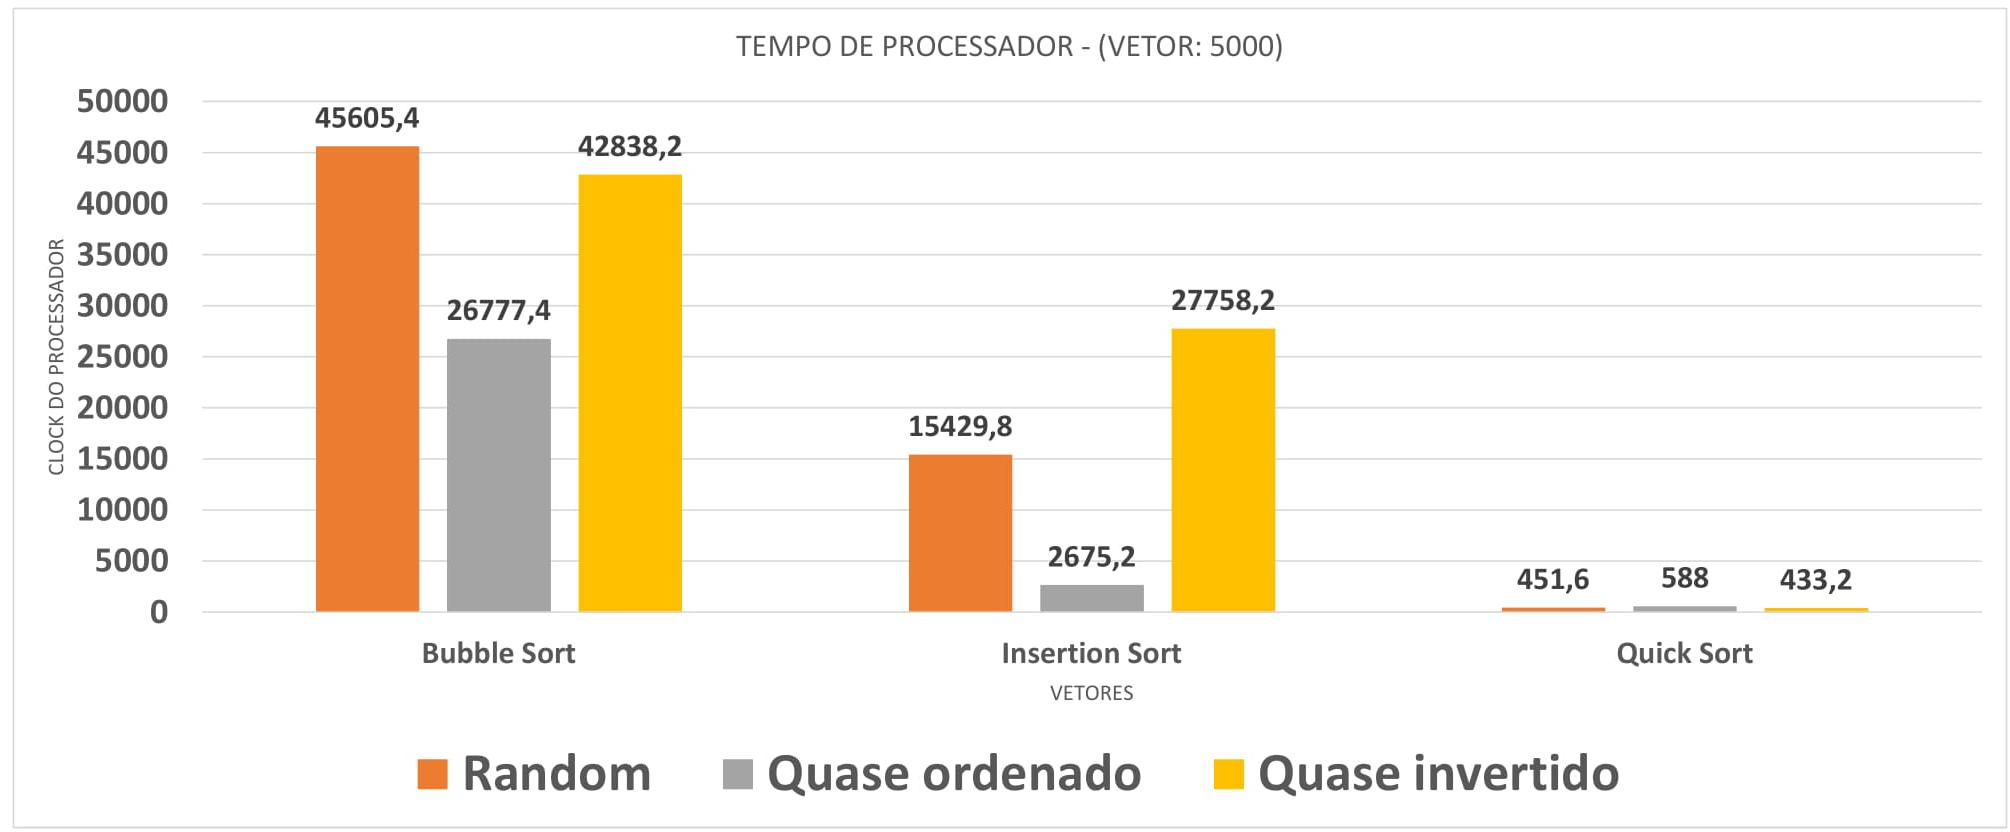
\includegraphics[width=15cm, height=6cm]{graficos/tempo_de_processador_random5-1.jpg}
     \caption{Gráfico tempo de processador (5000)}
     \label{T5}

     \centering
     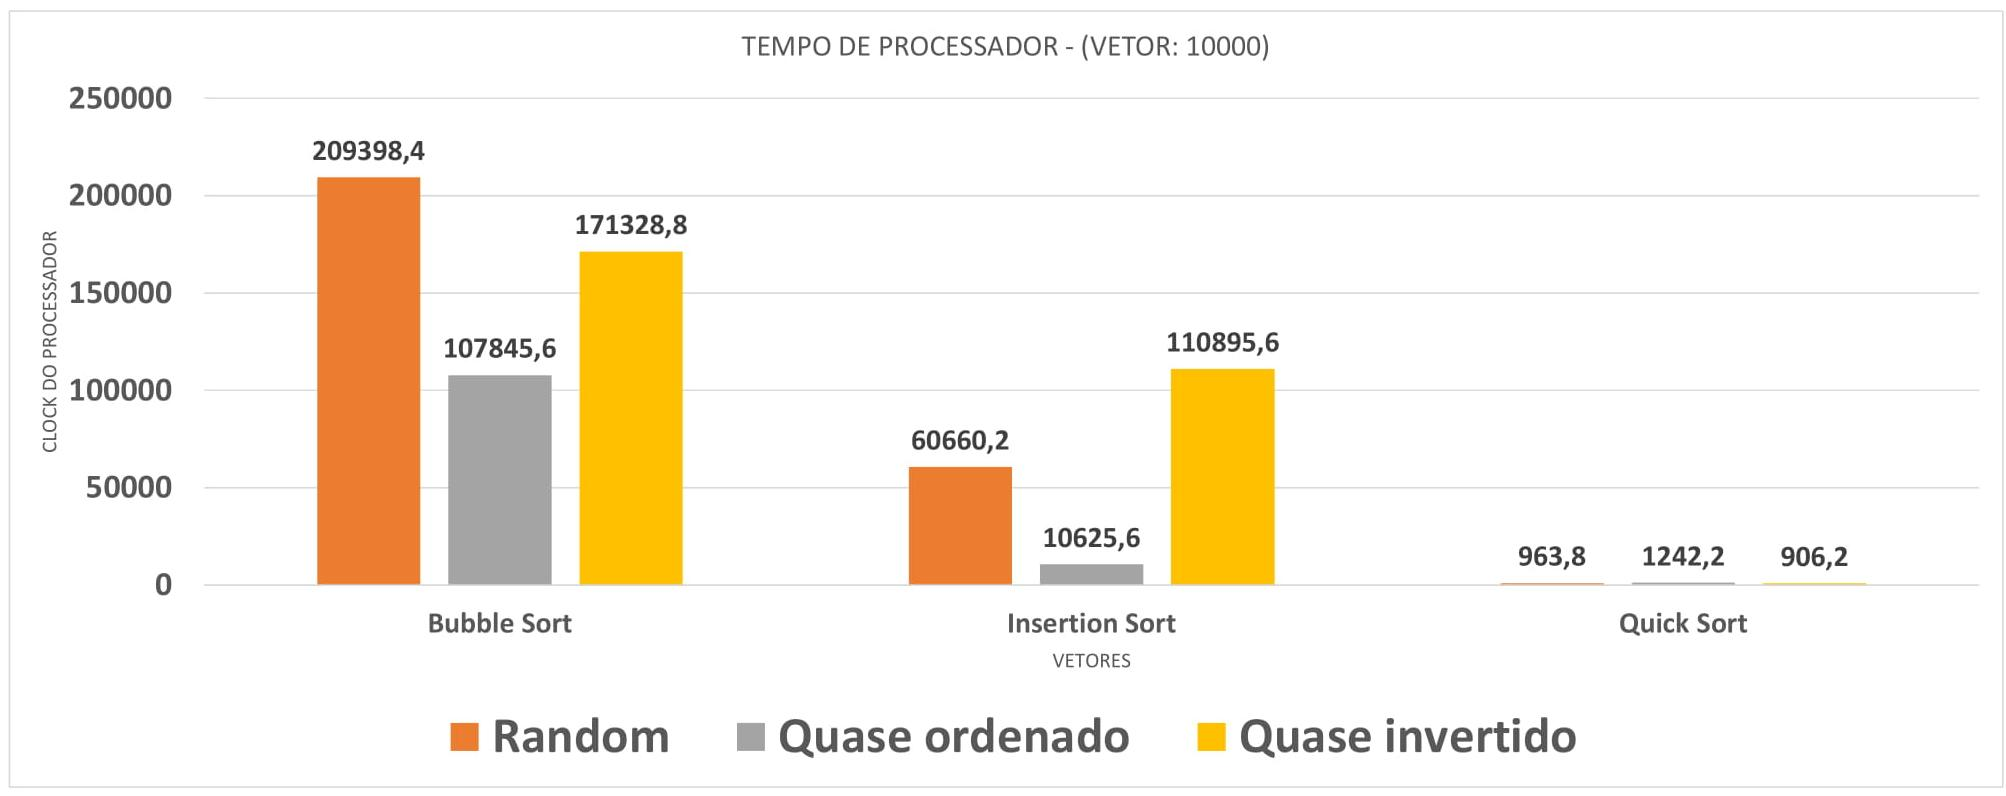
\includegraphics[width=15cm, height=6cm]{graficos/tempo_de_processador_random10-1.jpg}
     \caption{Gráfico tempo de processador (10000)}
     \label{T10}

     \centering
     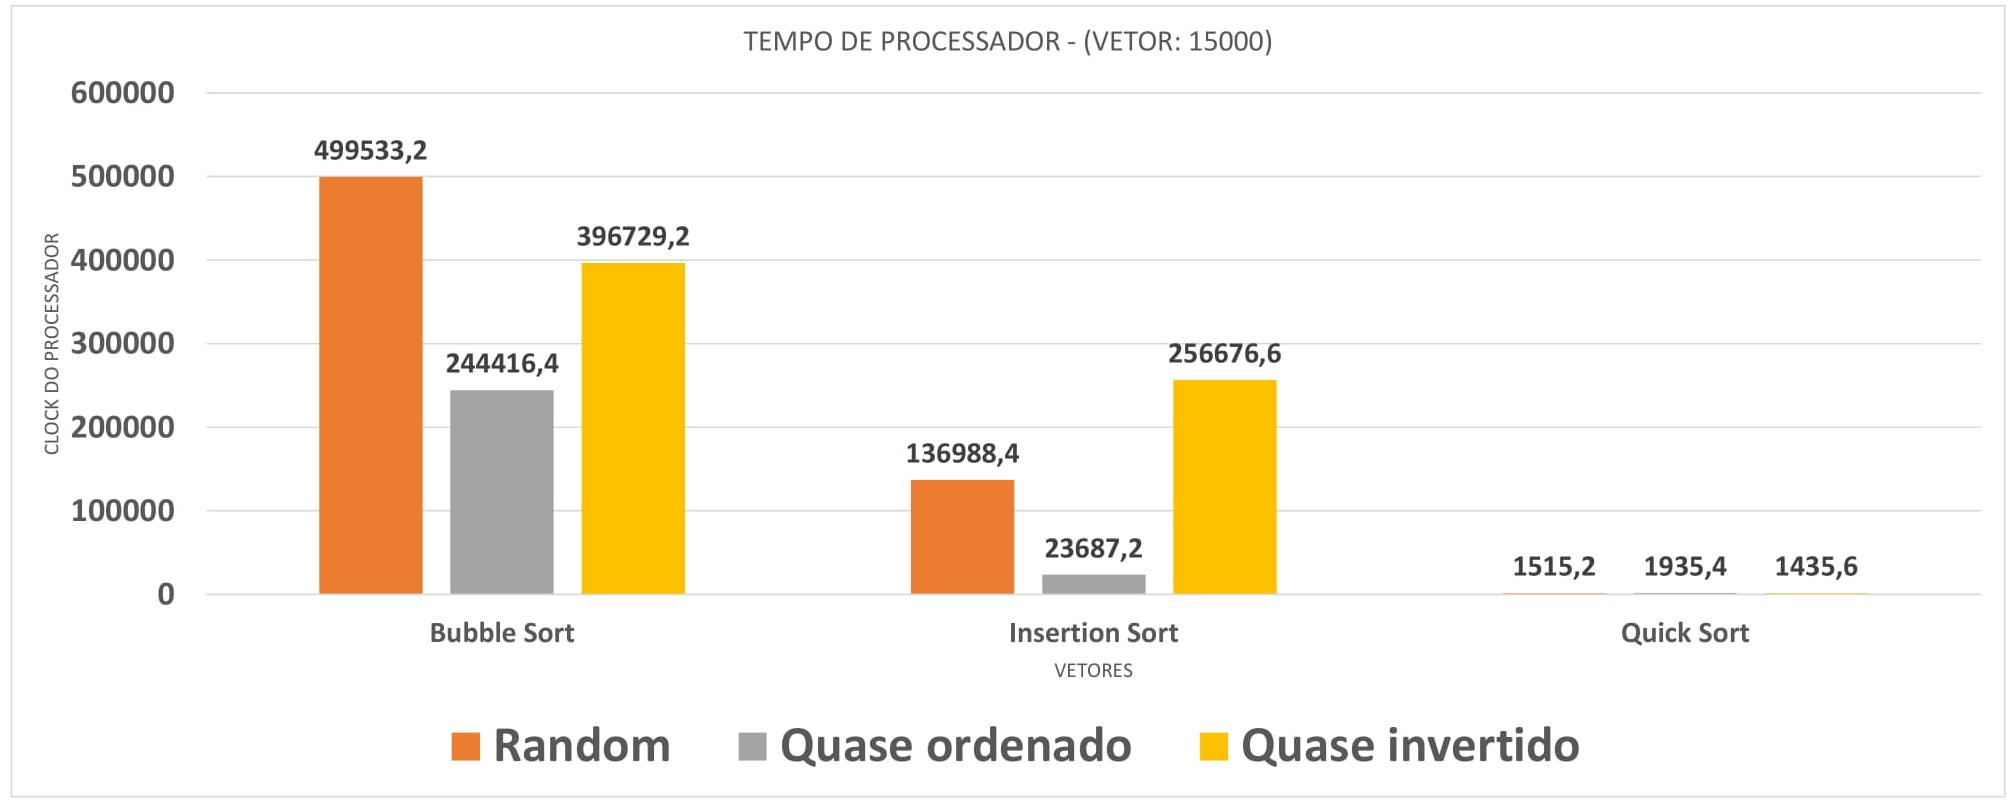
\includegraphics[width=15cm, height=6cm]{graficos/tempo_de_processador_random15-1.jpg}
     \caption{Gráfico tempo de processador (15000)}
     \label{T15}
\end{figure}

	

\begin{figure}[!htb]
     \centering
     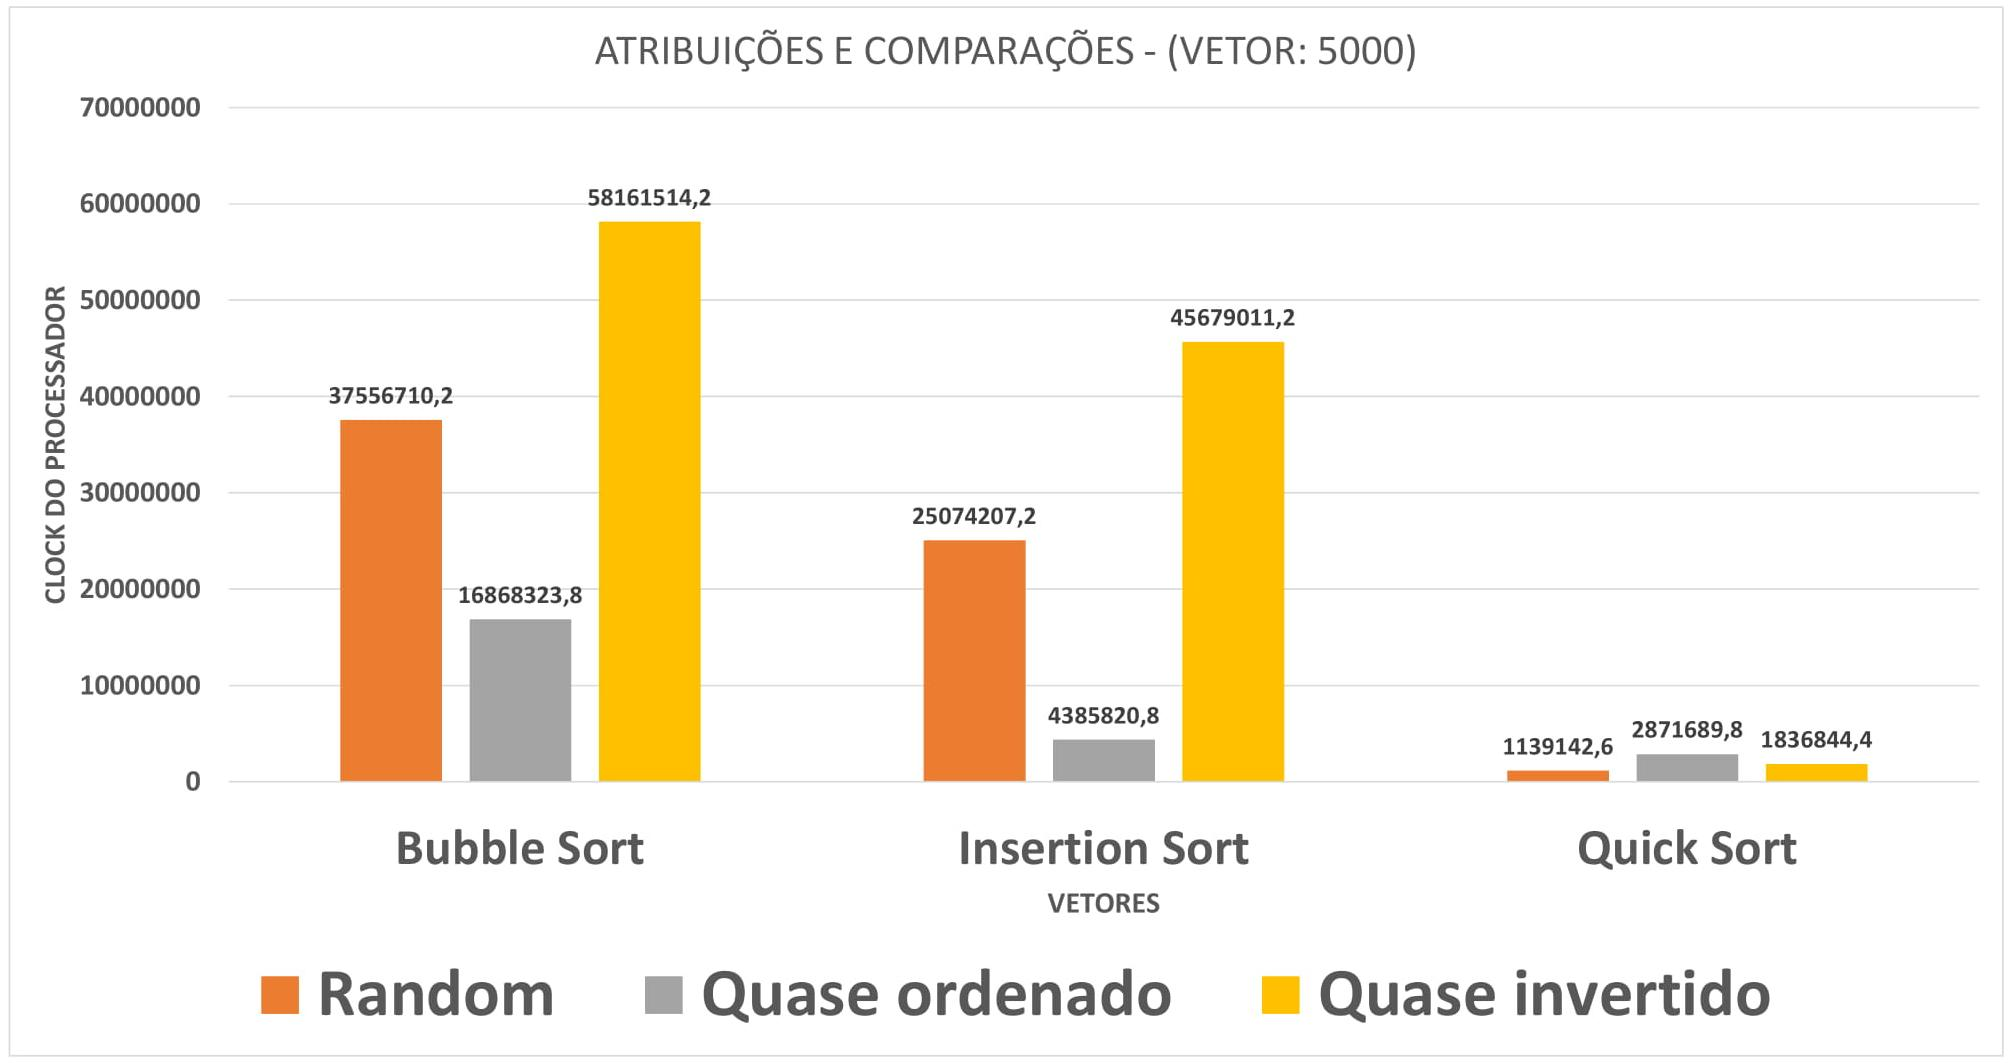
\includegraphics[width=15cm, height=6cm]{graficos/grafico_atribuicoes5-1.jpg}
     \caption{Gráfico atribuições e comparações (5000)}
     \label{A5}

     \centering
     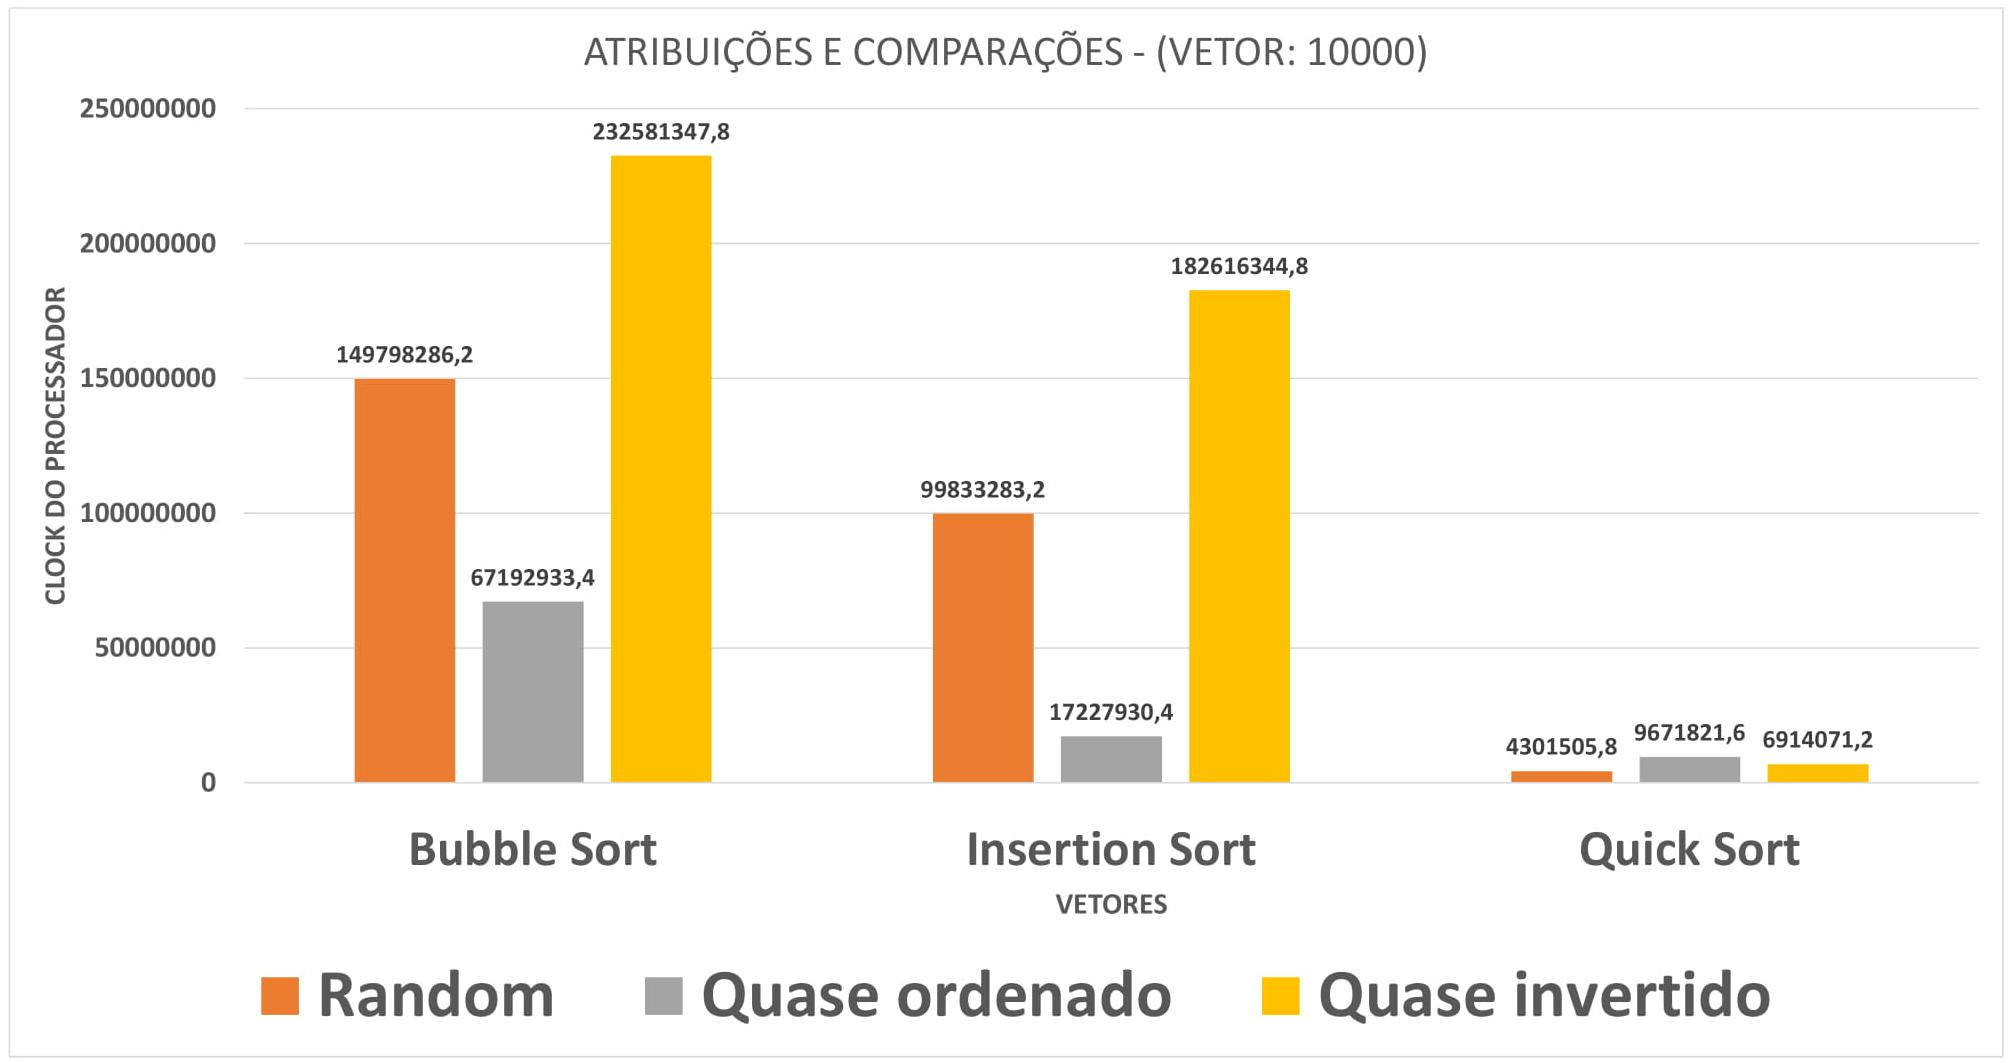
\includegraphics[width=15cm, height=6cm]{graficos/grafico_atribuicoes10-1.jpg}
     \caption{Gráfico atribuições e comparações (10000)}
     \label{A10}

     \centering
     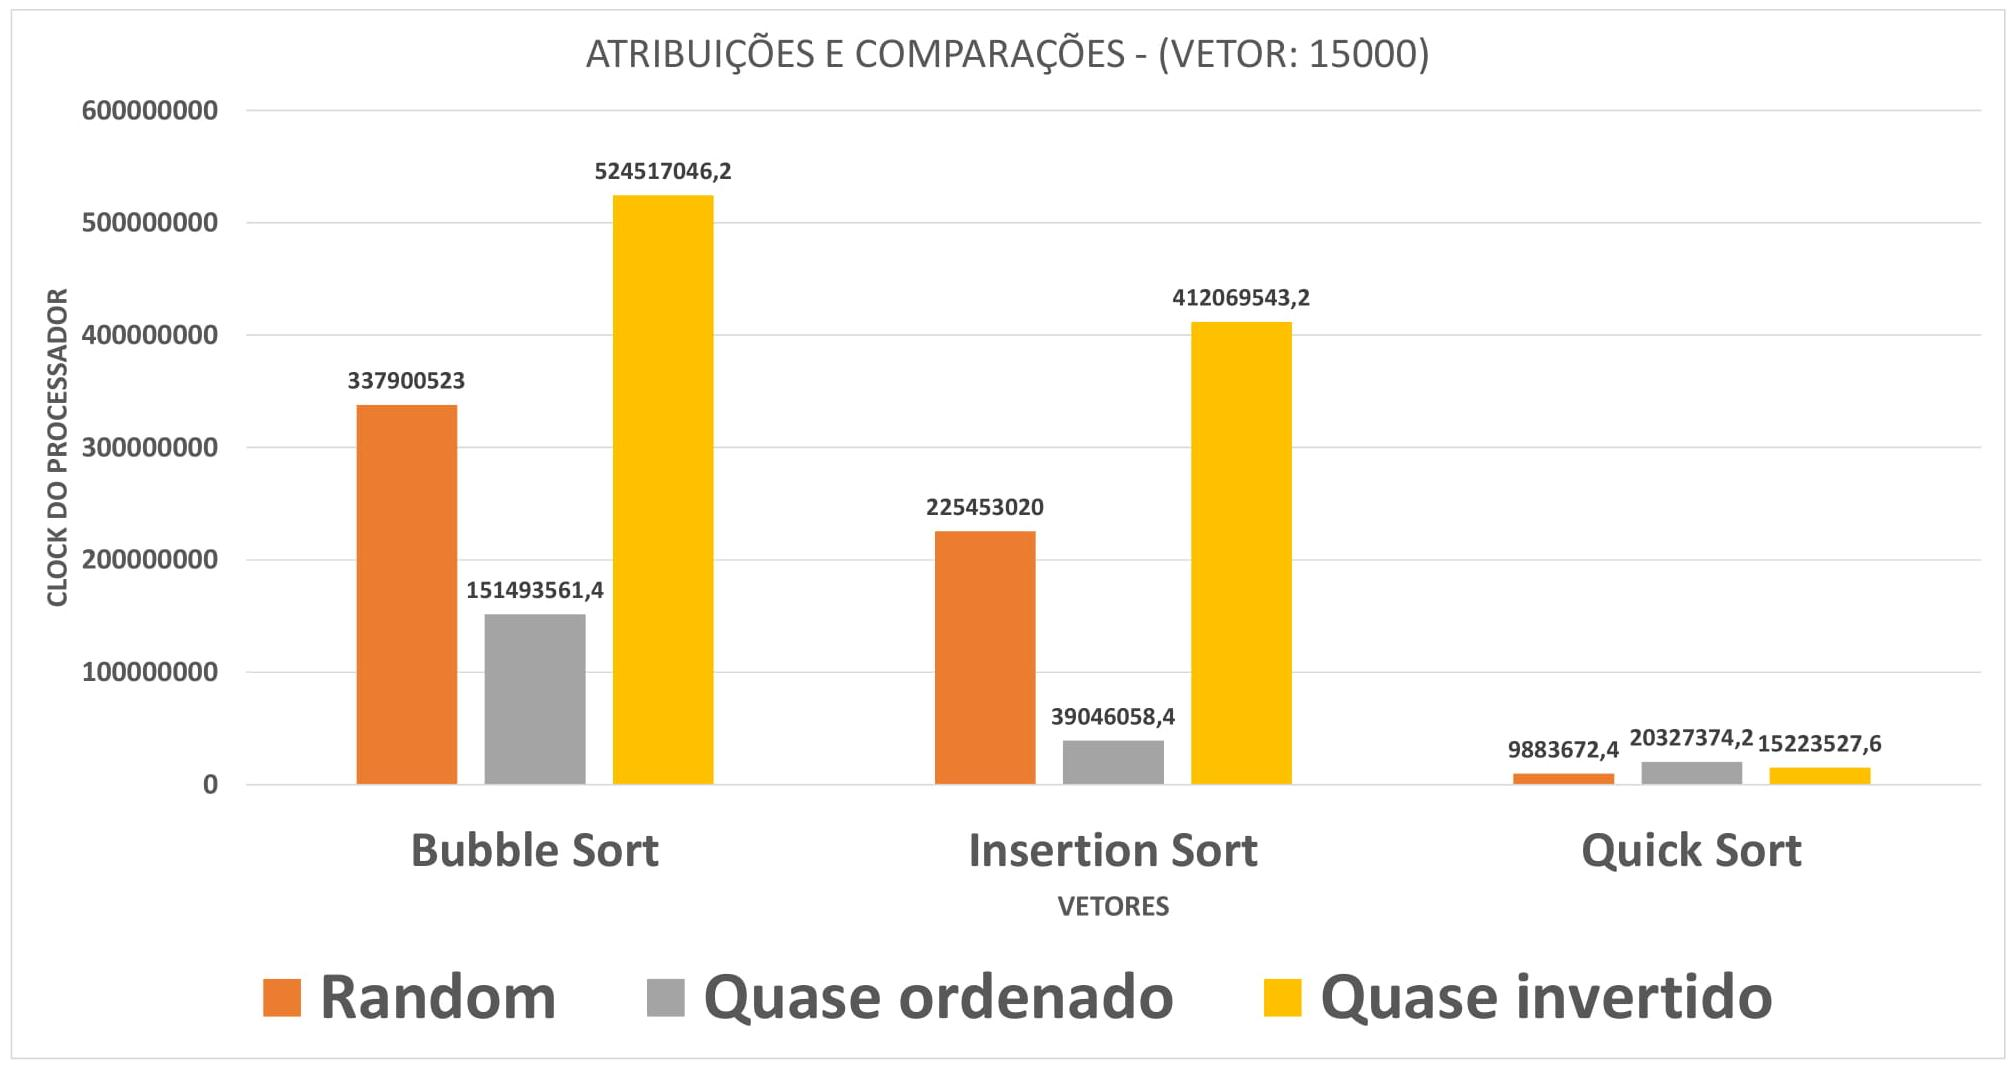
\includegraphics[width=15cm, height=6cm]{graficos/grafico_atribuicoes15-1.jpg}
     \caption{Gráfico atribuições e comparações(15000)}
     \label{A15}
\end{figure}

\newpage 
\section{Considerações Finais}




A análise sobre os resultados processados permitiu avaliar: que para todos os vetores independemente do tamanho ou sua configuração inicial Quick Sort prevaleceu como melhor tanto em desempenho quanto em velocidade, tendo seu pior caso sempre o vetor quase ordenado diferente dos demais algoritmos que tiveram ambos como melhor caso os vetores quase ordenados e seu melhor caso foram com os vetores quase invertido.

O segundo melhor algoritmo foi o Insertion Sort que como foi dito antes seu melhor caso para os vetores de todos os tamanhos foi os quase ordenados e seu pior caso foi quase invertido.

Por ultimo temos o Bubble Sort que saiu como algoritmos mais lento e com mais atribuições e comparações em todos casos seu melhor caso foi com os vetores quase ordenados e o pior caso com os vetores aleatórios.



\bibliographystyle{sbc}
\bibliography{sbc-template}

\end{document}
\grid
\grid
\grid
\grid
